\chapter{Background and Related Work}
\label{Chapter1}

\textbf{Procedural terrain generation} refers to the algorithmic creation of terrains, as opposed to manually modelling them. This approach has gained significant popularity in video games, simulations, and virtual reality environments due to its ability to create vast, detailed landscapes efficiently. In this chapter, we explore the foundations of procedural terrain generation, examining current methods and their limitations when integrating \textbf{fixed height constraints}.

Our research is implemented as a practical system within Unity, a widely-used game engine that provides robust terrain editing capabilities \citep{UnityTerrainDocs}. Throughout this thesis, we reference our Unity-based implementation to ground theoretical concepts in practical application.

\section{Procedural Terrain Generation Fundamentals}
\label{ptg_fundamentals}

The primary appeal of procedural generation lies in its capability to produce vast, detailed terrains without storing enormous amounts of explicit data of the terrain. Instead, these methods use algorithms and mathematical functions to generate terrain features \textit{on the fly} or \textit{during} the environment design process. This approach offers several advantages over manual terrain modelling; for example, these procedural methods can generate terrains of practically unlimited size and detail, making them very scalable. On top of this, with appropriate parameter adjustments, a single algorithm can produce plenty of unique terrain variations. It achieves this while still being memory efficient, as the explicit terrain heights and data do not need to be stored, only the \textit{appropriate code} to run the procedural terrain generation algorithm is necessary.

A key challenge in procedural terrain generation is mimicking the irregular patterns found in natural landscapes. Our system implements several foundational method, such as, Perlin noise with fractional Brownian motion, Voronoi-based generation, midpoint displacement, and erosion simulation. We will describe these in detail in the following sections.

\subsection{Perlin Noise}
\label{noise_based}

\textbf{Perlin noise} is the most fundamental technique in procedural terrain generation. Introduced by \textcite{Perlin85}, Perlin noise generates natural-looking patterns that are essential for creating believable landscapes. Unlike random noise, which produces abrupt discontinuities, Perlin noise ensures \textbf{smooth}, \textbf{continuous} variations between neighbouring points. 

The algorithm works by placing random gradient vectors at the corners of a grid, then calculating how strongly each corner's gradient influences any given point within that grid. These influences are blended together, producing \textit{gentle transitions} between points, rather than sudden jumps in height. This continuity makes Perlin noise particularly well-suited for natural terrain features such as hills, valleys, and rolling landscapes.


A more mathematical formulation of Perlin noise is as follows:

\[Perlin(x)=lerp(t,g_0 \times (x - x_0), g_1 \times (x - x_1))
\]

Where:
\begin{itemize}
    \item \(x_0\) and \(x_1\) are grid points surrounding \(x\);
    \item \(g_0\) and \(g_1\) are gradient vectors at those grind points;
    \item \(t=fade(x-x_0)\) is a \textit{smoothstep} function to ease the interpolation;
    \item \(lerp=(t,a,b)\) is linear interpolation between $a$ and $b$ using $t$.
\end{itemize}

We can see the effectiveness of Perlin noise in Fig. \ref{fig:noise_comparison} below, where white noise appears chaotic and discontinuous, while Perlin noise produces the smooth, gradual transitions essential for realistic terrain generation:

\begin{figure}[h]
    \centering
    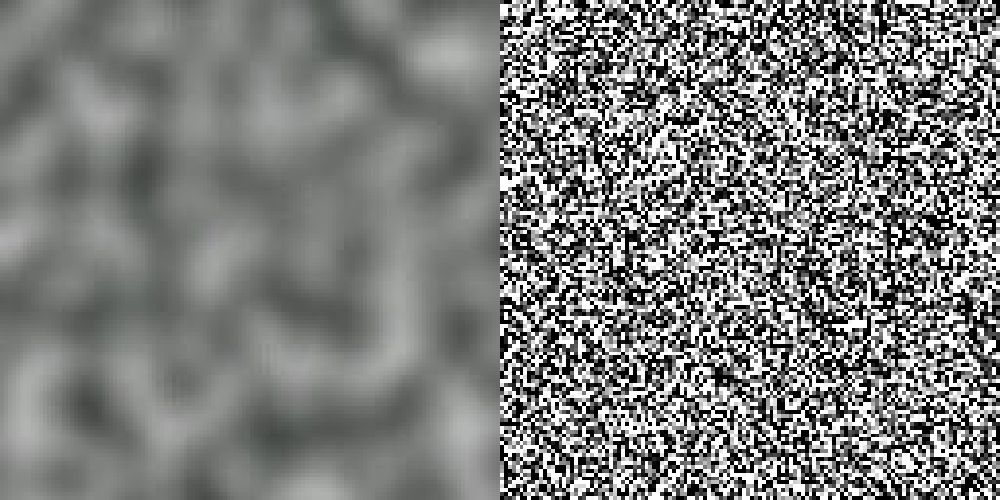
\includegraphics[width=0.6\textwidth]{img/PTG_fundamentals/noise_comparison.jpg}
    \caption{Comparison between Perlin Noise (left) and white noise (right). Image adapted from \cite{Geere2023}.}
    \label{fig:noise_comparison}
\end{figure}


\subsubsection{Fractional Brownian Motion (fBM)}

While basic Perlin noise creates smooth terrain variations, real-world landscapes exhibit detail at multiple scales simultaneously, from large mountain ranges down to small surface textures. \textbf{Fractional Brownian Motion (fBM)} addresses this limitation by combining multiple layers of noise at different scales to create more complex, naturalistic patterns, as described in ``Fractional Brownian Motion'' \citep{Inigo22}.

The fBM technique works by accumulating several layers (known as \textbf{octaves} in the literature) of noise, where each octave operates at a different frequency and amplitude:

\[\fBM(x) = \sum_{i=0}^{n-1} a_i \times \noise(f_i \times x)\]

Where:
\begin{itemize}
    \item $n$ is the number of octaves;
    \item $f_i$ represents the frequency multiplier for octave $i$ (typically $f_i = 2^i$);
    \item $a_i$ represents the amplitude for octave $i$ (typically $a_i = a_0 \times \text{persistence}^i$).
\end{itemize}

Each successive octave typically doubles the frequency while reducing the amplitude according to a persistence parameter. For example, with persistence = 0.5, each octave contributes half the amplitude of the previous one. Higher persistence values (closer to 1.0) preserve more detail in successive octaves, creating rougher, more complex terrain.

These noise-based functions lack inherent mechanisms to adapt their output to match specific height values at particular locations, often resulting in unrealistic cliff formations or abrupt slope changes \footnote{We address this limitation through a distance-based modification system in Chapter \ref{Chapter3}.}.

\subsection{Voronoi-Based Terrain Generation}
\label{voronoi_diagrams}

\textbf{Voronoi diagrams} partition space into regions based on \textit{distance} to a set of random points. It can form the basis of different types of terrains, like valleys, ridges, or islands, or it can produce full, complex terrains all by itself as seen in the paper \citetitle{Olsen04} by \textcite{Olsen04}. 

This technique starts by setting random points around the terrain and assigning random heights within a specified range. Then, for each pixel in the terrain, we calculate its distance to all peaks and set the height based on the nearest peak, then applying a \textit{falloff} function to create smooth hills. The falloff function determines how terrain height decreases with distance from each peak. 

A typical falloff function takes the form:

\[h(d) = h_{peak} \times \max(0, 1 - (\frac{d}{r})^p) \]
Where:
\begin{itemize}
    \item $h_{peak}$ is the peak's height;
    \item $d$ is the distance from the peak;
    \item $r$ is the peak's radius of influence;
    \item $p$ is a power parameter controlling the falloff curve shape. When $p = 1$, this creates a linear cone; $p = 2$ produces a smoother, parabolic hill; and higher values create flatter tops with steeper sides. 
\end{itemize}

\subsection{Midpoint Displacement}
\label{midpoint_displacement}

The \textbf{midpoint displacement} algorithm, also known as the \textbf{diamond-square} algorithm, is one of the earliest and most intuitive approaches to procedural terrain generation \citep{Olsen04}. The algorithm is a recursive method for generating terrain by progressively refining the grid of elevation values. The rough outline of the method is as follows:

\begin{itemize}
    \item[-] We begin by setting initial heights at the four corners of the grid;
    \item[-]  Then, in the \textit{diamond} step, we calculate the centre point (\textbf{midpoint}) of a square by averaging the values of the corners and adding a small random offset to create natural variation;
    \item[-] Next, in the \textit{square} step, we do the same for the midpoints of each edge; 
    \item[-] The grid is then subdivided into smaller squares, and we repeat the process on each one, gradually adding more detail to the terrain.
\end{itemize}

The diamond-square algorithm's recursive nature makes it particularly interesting from both theoretical and practical perspectives. What fascinates us about this approach is how it builds complexity through \textit{progressive refinement}, starting with broad terrain features and gradually adding finer detail. The algorithm's inherent respect for spatial relationships means that neighbouring points influence each other naturally, creating the smooth transitions essential for believable terrain.

\subsection{Erosion}
\label{erosion_1}

While noise-based and geometric algorithms form the foundation of procedural terrain generation, erosion simulations play a vital role in adding realism by mimicking natural weathering processes (this refers to the breakdown and alteration of rocks and soil through physical or chemical means, shaping landscapes over time). In terrain generation, two primary types of erosion are commonly simulated to reproduce these effects: 

\subsubsection{Hydraulic Erosion}
\label{hydra_erosion}
This technique simulates how water shapes the terrain over time, forming features like river valleys, gullies, and deltas. Our implementation follows the approach described by Olsen \citep{Olsen04}, where rain is simulated by randomly placing water droplets across the terrain. Each droplet dissolves (erodes) part of the surface, then flows downhill, carrying sediment with it. As the droplet moves, some of the water evaporates, diminishing its effect. 

The algorithm's strength lies in its particle-based approach, where each droplet follows a path of steepest descent, eroding terrain along its journey until its erosive power is depleted. This creates the valley networks we observe in nature, where water naturally carves channels that converge into larger drainage systems.

To view the actual pseudocode of the algorithm, please see the appendix \ref{alg:hydraulic_erosion}

\subsubsection{Thermal Erosion}
\label{thermal_erosion}
This algorithm identifies slopes that exceed a specified angle and redistributes the material to lower cells until a suitable level of stability is achieved. This process softens sharp slopes, such as mountain peaks or cliffs, resulting in terrain that closer resembles those in the real world. What makes this algorithm particularly effective is its consideration of material conservation, when sediment erodes from steep slopes, it must be deposited somewhere else, typically in adjacent lower areas. 

For the pseudocode of the algorithm, see the appendix \ref{alg:thermal_erosion}.

\section{Heightmap-Based Terrain Representation}

Another relevant topic we would like to discuss is a \textbf{heightmap-based representation} of landscapes. Heightmaps represent terrain as a \textit{two-dimensional grid} where each cell stores an \textbf{elevation value} mapping to the corresponding pixel height. This representation offers several advantages, such as memory efficiency and simplicity of modification and rendering. Typically, heightmaps are stored as greyscale images,  where brightness corresponds to elevation (an example can be seen in Fig. \ref{fig:noise_comparison}), or two-dimensional arrays of floating-point values between 0 (minimum height) and 1 (maximum height). 

This approach does, however, sacrifice the ability to represent overhangs and caves, as each cell of the terrain can only have exactly one height. Unity's terrain system \citep{UnityTerrainDocs} utilises heightmaps as its primary terrain representation, and this, along with its simplicity, is why we went with this representation in our thesis. This representation is particularly suitable for working with constraint masks that identify fixed points, which forms the foundation of our approach in Section \ref{terrain_system_integration}.

\section{Constrained Procedural Generation}

To start this section off, we illustrate in figure \ref{fig:constraint_discontinuity} a fundamental challenge in constrained procedural terrain generation, namely the \textbf{boundary problem}. 

\begin{figure}[h!]
    \centering
    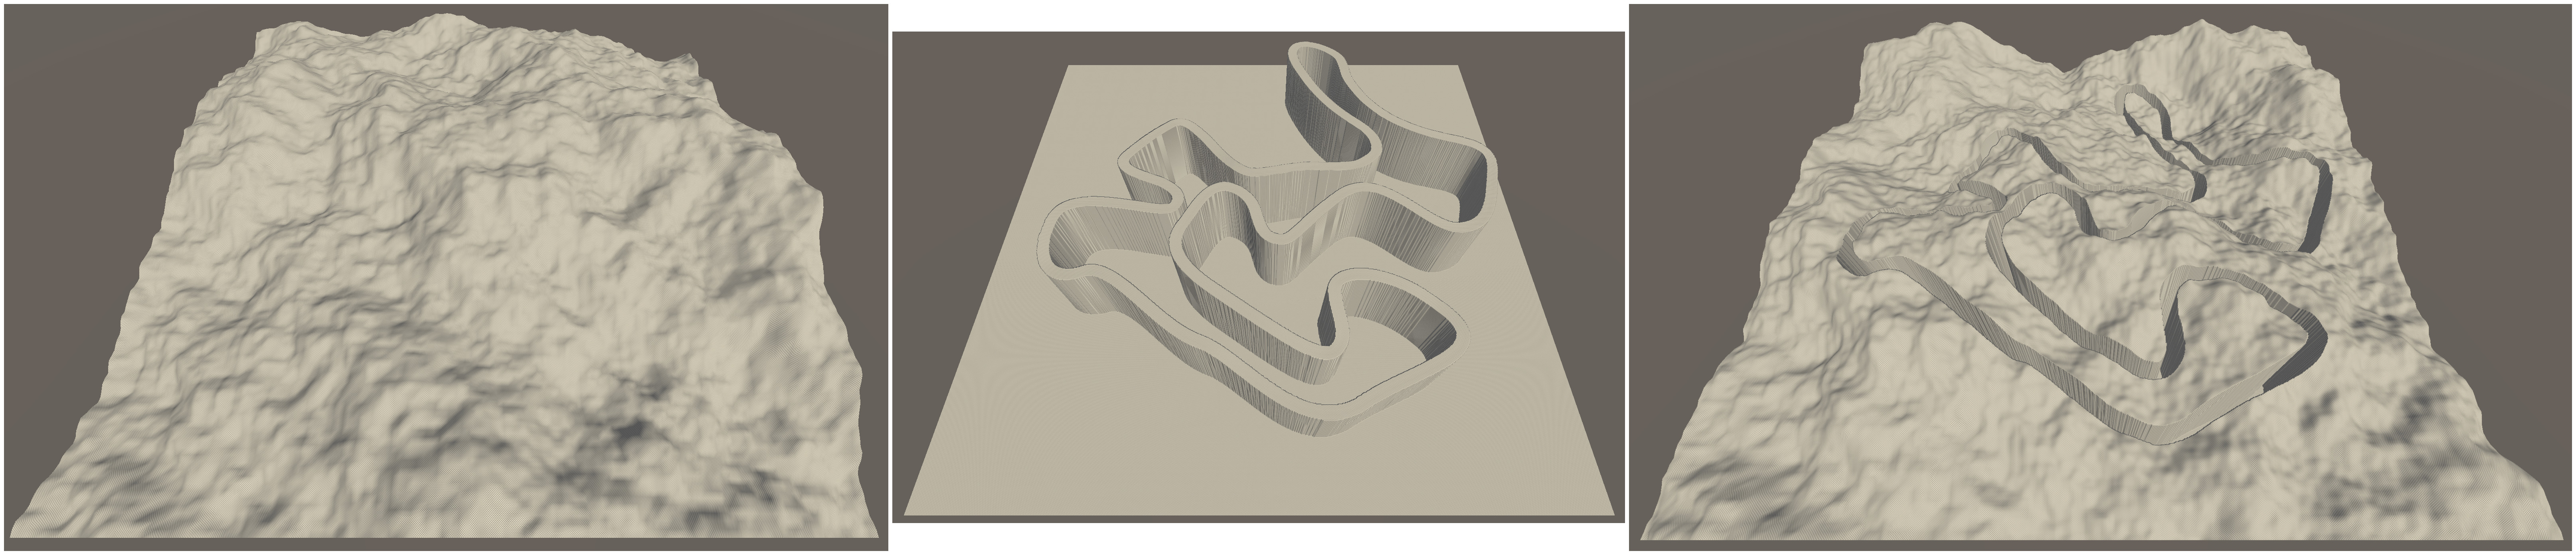
\includegraphics[width=1.0\textwidth]{img/discontinuity_example.jpg}
    \caption{Conceptual illustration of the boundary problem in constrained procedural generation. (Left) Unconstrained terrain generated with Perlin noise. (Centre) Fixed height constraints embedded in the terrain. (Right) The resulting discontinuities that appear at the boundaries between fixed and procedurally generated areas.}
    \label{fig:constraint_discontinuity}
\end{figure}

When we place fixed height areas inside generated terrain without proper blending, obvious breaks appear where they meet. These artifacts destroy the visual coherence of the terrain and create unrealistic formations, like sudden cliffs or unnatural slopes. Developing techniques to address this boundary problem is a central focus of our research.


\subsection{Previous Approaches to Constrained Generation}

Conventional procedural terrain generation typically starts from a flat surface and then populates the heightmap with elevations derived from generative algorithms, such as Perlin noise and midpoint displacement. The output of the algorithm is controlled by fine-tuning various parameters (for example, the maximum height allowed), but overall does not allow for very precise control.  This is where many have used the concept of \textit{constrained procedural generation}. These approaches do not necessarily tackle the exact same problem as we intend to, where these constraints are the fixed heights of any areas in the terrain. Rather, they tend to be more \textit{specific} to a type of constraint, such as generating surrounding terrain for a \textbf{predefined} river network. We will now discuss current existing solutions to this problem. 

\subsubsection{The Bottom-Up Method}
\label{bottom_up_method}

The \textbf{bottom-up approach} for procedural generation, described by \textcite{Belhadj07,} starts with the constraints themselves as the foundation for terrain growth, building \textit{outward} from these fixed points. This method is designed to work well when constraints form connected patterns like river networks or ridge lines, as these constraint types are continuous paths through the terrain rather than isolated points.

This solution works by storing the heights and areas of the river network in a digital heightmap while all other points remain to be computed afterwards. To address the boundary problem, \textcite{Belhadj07} developed their novel \textbf{Midpoint Displacement Inverse (MDI)} process, which inverts the traditional midpoint displacement operation to propagate height information outwards from the fixed points, creating smooth transitions to the surrounding procedurally generated terrain.

While this approach produces realistic terrain without discontinuities, it may not work well with \textbf{isolated fixed points}. Additionally, the method is tailored to midpoint displacement and does not readily apply to other procedural terrain generation methods. 

\subsubsection{Path-Based Constraint Methods}
\label{path_based_method}

Another method addressing the constraint problem is described in the paper  \citetitle{Andereck14}, where the author focuses specifically on \textbf{path constraints}. In this work, \textit{user-defined paths} with exact height constraints serve as the foundation for terrain generation. Unlike approaches that may modify constraints slightly for better terrain coherence, this method preserves the exact heights of predefined paths while procedurally generating surrounding terrain features.

The algorithm employs a data structure that works with multiple different scales. At each scale of the data structure, the algorithm fits planes to constraint points using least-squares fitting, ensuring the terrain naturally conforms to the paths while maintaining realistic slopes. This creates terrain that respects path heights while achieving smooth transitions to the surrounding areas.

This approach works particularly well for path-like constraints but is less suitable for \textbf{arbitrary} fixed areas or disconnected constraint patterns \footnote{We will demonstrate a comparison between our approach and both bottom-up and path-based methods in Chapter \ref{Chapter5}.}.

While these constrained generation methods provide mechanisms for integrating fixed height areas with procedurally generated terrain, they introduce an additional layer of complexity that extends beyond the boundary problem itself. Each technique requires careful parameter tuning to achieve natural-looking results, and when multiple techniques are combined in complex pipelines, the parameter optimisation challenge becomes a significant barrier to practical adoption. The following section examines this fundamental challenge and explores algorithmic approaches for addressing it.

\section{Parameter Optimisation in Procedural Generation}
\label{parameter_optimization}

While constrained procedural generation methods provide mechanisms for integrating fixed height areas with generated terrain, they introduce a fundamental challenge that extends beyond the boundary problem: \textbf{parameter optimisation}. Each terrain generation technique brings its own set of parameters that must be carefully tuned to achieve desired results. When these techniques are combined in complex pipelines, the parameter space becomes vast and interconnected, creating a significant barrier to effective terrain generation.

Consider a typical terrain generation pipeline that might include Perlin noise (requiring frequency, octaves, persistence, and amplitude parameters), Voronoi-based mountain generation (needing peak count, falloff rates, and height ranges), multiple smoothing operations (each with iteration counts and strength parameters), and erosion simulations (requiring threshold values and erosion rates). When these operations are chained together, the parameter space becomes \textbf{exponentially complex}, with small changes in one parameter often requiring adjustments throughout the entire pipeline to maintain natural-looking results.

This parameter complexity represents one of the most significant practical challenges in procedural content generation. Traditional approaches require either expert domain knowledge for manual tuning or mathematical fitness functions for automated optimisation, both of which are problematic when the goal is subjective terrain quality that depends on aesthetic preferences rather than quantifiable metrics.

\subsection{The Parameter Space Challenge}
\label{parameter_space_challenge}

The complexity of parameter tuning in procedural terrain generation manifests in several ways. \textbf{Parameter interdependency} means that adjusting one parameter often requires compensatory changes throughout the system. For example, increasing noise amplitude might necessitate stronger erosion and different smoothing parameters to maintain realistic terrain characteristics. This makes systematic exploration difficult and counter-intuitive. Furthermore, \textbf{subjective quality assessment} presents a fundamental difficulty. Unlike optimisation problems with clear mathematical objectives, terrain quality is \textit{inherently} aesthetic and context-dependent. What constitutes "natural" or "appealing" terrain varies significantly based on the intended application, user preferences, and specific environmental context.


These challenges motivate the need for alternative optimisation approaches that can navigate complex parameter spaces while incorporating human aesthetic judgment. Genetic algorithms, particularly in their interactive variants, provide a promising framework.

\subsection{Genetic Algorithms: Fundamentals}
\label{genetic_algorithms_fundamentals}

\textbf{Genetic algorithms} (GAs) represent a class of evolutionary computation techniques that mimic the process of natural selection to solve optimisation and search problems. Unlike traditional methods that rely on gradient information, GAs maintain a \textbf{population} of candidate solutions and evolve them through \textbf{selection}, \textbf{crossover}, and \textbf{mutation}.

In terrain generation, an \textbf{individual} (of the population) might represent a \textit{specific combination} of algorithm parameters. Additionally: 

\begin{itemize}
    \item The \textbf{fitness function} measures \textit{how well} an individual solves the problem. Higher-fitness individuals are more likely to be selected for reproduction; 
    \item \textbf{Elitism} ensures the best individuals are preserved throughout the whole evolutionary process;
    \item \textbf{Crossover} combines traits from parents;
    \item \textbf{Mutation} introduces random variations in the individuals.
\end{itemize}

One complete cycle of the algorithm consists of all these features (usually ordered as: evaluation, selection, crossover, and mutation). The algorithm iterates through multiple generations, with the population gradually improving over time.

\subsection{Interactive Genetic Algorithms}
\label{interactive_genetic_algorithms}

While traditional genetic algorithms rely on mathematical fitness functions, many creative and design problems, including terrain generation, involve subjective quality criteria that resist formal mathematical description. \textbf{Interactive Genetic Algorithms} (IGAs) address this limitation by replacing automated fitness evaluation with \textbf{human judgment}, transforming the optimisation process into a collaborative exploration between human creativity and algorithmic efficiency. 


Interactive genetic algorithms also introduce unique challenges that distinguish them from traditional automated approaches. Human evaluation is limited by attention span and cognitive load, so IGA systems must balance population size and generation length to avoid user fatigue. A common approach is to let users select multiple preferred individuals, instead of scoring each one numerically.

The IGA approach has been applied to terrain generation by \textcite{Walsh10}, who developed a system where users evolved terrain through visual selection. Their work demonstrated that users could discover appealing parameter combinations without needing detailed technical knowledge. 


\hfill

Inspired by this work and motivated by existing challenges and limitations, we build on this framework and present our solution via an interactive genetic algorithm in Chapter \ref{Chapter4}. Together, these innovations provide a practical and efficient method for procedural terrain generation with fixed height constraints.


